\documentclass[11pt]{article}
\usepackage[utf8]{inputenc}
\usepackage{geometry}
\usepackage{graphicx}
\usepackage{hyperref}
\usepackage{amsmath}
\usepackage{amsfonts}
\usepackage{amssymb}
\usepackage{color}
\usepackage[capitalise,noabbrev]{cleveref}
\usepackage{caption}
\usepackage{subcaption}
\geometry{a4paper}

\title{MuesliSwap Open Transaction Chaining \\--- Project Closeout Report ---}
\author{MuesliSwapTeam}
\date{\today}

\begin{document}


\maketitle


\section*{Official Close-Out Summary}
\begin{itemize}
    \item \textbf{Name of project and Project URL on Fund:}\\
    MuesliSwap Open Transaction Chaining \\
    \url{https://projectcatalyst.io/funds/10/f10-development-and-infrastructure/open-transaction-chaining-tooling-to-speed-up-cardano-dapps-by-muesliswap}

    \item \textbf{Project ID:} 1000139

    \item \textbf{Project managed by:} MuesliSwap Team

    \item \textbf{Project started in:} November 2023

    \item \textbf{Project completed in:} November 2024

    \item \textbf{Challenge KPIs and how the project addressed them:}
    \begin{itemize}
        \item \textbf{Faster dApp interactions:} Implemented TxChaining in Nami Wallet, allowing dependent transactions to be chained without waiting for on-chain confirmation.
        \item \textbf{Improved developer experience:} Provided code, documentation, and examples (PyCardano, \texttt{ogmios}, \texttt{Blockfrost}) to guide developers in using TxChaining.
        \item \textbf{Validation of concept:} Demonstrated on-chain test transactions on PreProd, confirming multiple chained transactions could appear in a single block.
    \end{itemize}

    \item \textbf{Project KPIs and how the project addressed them:}
    \begin{itemize}
        \item \textbf{Implement TxChaining in Nami Wallet:} Integrated \texttt{getMempoolTxs} and Mempool History features, enabling real-time referencing of pending transactions.
        \item \textbf{Demonstrate working TxChaining on PreProd testnet:} Showed successful chained transactions confirmed in the same block.
        \item \textbf{Close-out communication and demo:} Produced this close-out report, a video demonstration, and engaged with the community.
        \item \textbf{Community documentation and engagement:} Shared results via repositories, social media, and live discussions, encouraging feedback and adoption.
    \end{itemize}

    \item \textbf{Key achievements:}
    \begin{itemize}
        \item Successfully implemented TxChaining in a popular Cardano wallet (Nami).
        \item Engaged with the Cardano community through open-source code, Twitter Spaces, and forums.
        \item Documented implementations and test results, fostering collaboration and understanding.
    \end{itemize}

    \item \textbf{Key learnings:}
    \begin{itemize}
        \item Cardano Node inherently supports TxChaining, so no node-level changes or CIP submissions were needed.
        \item Tools like \texttt{ogmios} and \texttt{Blockfrost} support TxChaining workflows effectively.
        \item Early community engagement helps refine focus and implementation strategies.
    \end{itemize}

    \item \textbf{Next steps for the product or service developed:}
    \begin{itemize}
        \item Encourage adoption of TxChaining by other wallets and dApps.
        \item Continue refining documentation, examples, and community education.
        \item Consider future standardization efforts or best practices for TxChaining references.
    \end{itemize}

    \item \textbf{Final thoughts/comments:}\\
    TxChaining enhances transaction efficiency and user experience for Cardano dApps. This project sets a foundational example and provides open-source resources, paving the way for broader ecosystem adoption and innovation.

    \item \textbf{Links to other relevant project sources or documents:}
    \begin{itemize}
        \item Custom Nami Wallet Implementation (PR):\\
        \url{https://github.com/input-output-hk/nami/pull/966}
        \item PyCardano Transaction Chaining Examples:\\
        \url{https://github.com/MuesliSwapTeam/muesliswap-transaction-chaining}
        \item X (Twitter) Space Community Discussion:\\
        \url{https://x.com/MuesliSwapTeam/status/1863674797986594842}
        \item Further Documentation:\\
        \url{https://github.com/MuesliSwapTeam/muesliswap-transaction-chaining/blob/main/report/main.pdf}
    \end{itemize}

    \item \textbf{Link to Close-out Video:} \url{https://www.youtube.com/watch?v=WdUY8CbxWDU}
\end{itemize}


\section{Introduction}
This report provides a summary and analysis of the MuesliSwap Open Transaction Chaining (TxChaining) project for the Cardano Catalyst. The goal of this project was to improve the transaction efficiency of Cardano-based decentralized applications (dApps) by implementing TxChaining capabilities in the Nami Wallet and assessing the support for TxChaining in the Cardano Node and related tools.

\section{Changes to Original Plan}
In the original project proposal, we anticipated making modifications to both the Cardano Node and Nami Wallet to support TxChaining. During the development process, however, we found that:

\begin{itemize}
    \item The Cardano Node already natively supports TxChaining, negating the need for direct modifications to the Node itself.
    \item Development efforts shifted towards ensuring compatibility and verifying support for TxChaining in tools that interact with the Node, specifically \texttt{ogmios} and \texttt{Blockfrost}.
\end{itemize}

The updated approach involved implementing TxChaining in the Nami Wallet and creating a custom demonstration using PyCardano, showcasing successful transaction chaining with these tools. This pivot allowed us to optimize our resources and focus on enhancing Nami Wallet’s functionalities with:

\begin{itemize}
    \item \texttt{getMempoolTxs} function, enabling real-time access to pending transactions.
    \item Mempool History support, allowing the wallet to track transaction statuses within the mempool.
\end{itemize}

Our changes also included a demo video demonstrating the txChaining version of the Nami Wallet, documentation of PyCardano tools for chained transactions, and example PreProd transactions illustrating successful TxChaining in a single block using both \texttt{ogmios} and \texttt{Blockfrost}.

\section{Project Achievements}
The project was completed across three milestones, each achieving significant progress towards implementing and validating TxChaining.

\subsection{Milestone 1: Initial Implementation Plan}
The initial milestone included planning and proposing implementation strategies for TxChaining in both the Cardano Node and Nami Wallet. A detailed report and CIP impact analysis were provided in the project’s public repository, laying the groundwork for the next stages.

\subsection{Milestone 2: TxChaining Integration in Nami Wallet and Demo Creation}
In this milestone, we focused on implementing TxChaining functionality in the Nami Wallet. Key deliverables included:

\begin{itemize}
    \item Integration of the \texttt{getMempoolTxs} and Mempool History tracking features within Nami Wallet.
    \item A demo video showing chained transactions using PyCardano tools, all of which appear in the same block, proving successful TxChaining.
    \item Example transactions completed in the PreProd environment that showcase successful chained transactions, all linked in the same block.
\end{itemize}

\subsection{Milestone 3: Finalization and Community Engagement}
The final milestone focused on testing, documenting, and sharing the results with the community. Notable accomplishments include:

\begin{itemize}
    \item Comprehensive testing and validation of TxChaining features in the Nami Wallet.
    \item Opened pull requests for the Nami Wallet, Cardano Node, and CIP repositories to submit the TxChaining implementations and proposed CIP modifications.
    \item Engaged the Cardano community through Twitter, Discord, and public forums, including a live Twitter Space and CIP discussions.
\end{itemize}

\section{Frontend Testing and Test Report}

To verify the successful implementation of transaction chaining (TxChaining) in the Nami Wallet, we conducted a detailed frontend testing process. This section describes the testing procedure, highlights the expected results at each step, and offers contextual insights into how these changes improve transaction functionality within the Cardano ecosystem.

\subsection{Test Procedure and Observations}

Our testing process involved creating a simple transaction in the modified version of the Nami Wallet, observing how pending transactions are handled, and validating the availability of transaction data before confirmation on-chain. This is especially valuable for high-frequency Cardano dApp interactions that require rapid transaction updates and chaining capability.

\begin{enumerate}
    \item \textbf{Initiating a Transaction in Nami Wallet}\\
    First, we open the modified version of the Nami Wallet and initiate a new transaction by clicking the \texttt{Send} button. This action opens the interface where we can specify transaction details, such as the recipient and amount. 
    \newline
    \begin{figure}[ht]
        \centering
        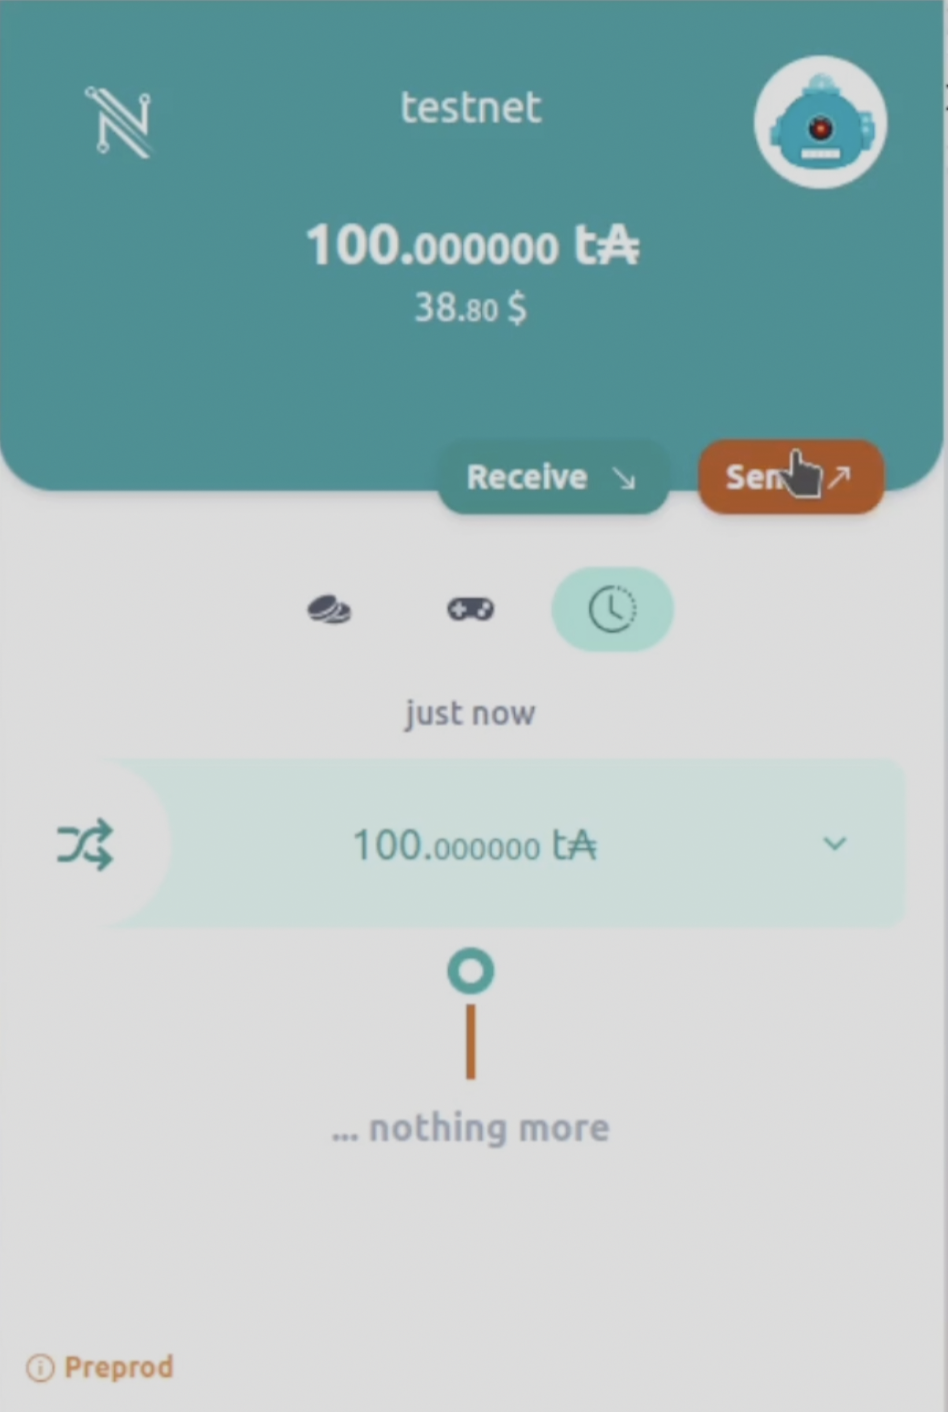
\includegraphics[width=100px]{./imgs/fe1}
        \caption{Nami Wallet Send Interface open, ready for transaction details input}
    \end{figure}
    
    \item \textbf{Specifying Transaction Details and Initiating Send}\\
    For this test, we specify a simple amount of Ada to send. While this test uses a straightforward transfer of Ada, it’s important to note that TxChaining also supports complex transaction contents, including smart contracts, token minting, and multi-input transfers. This versatility demonstrates the robustness of TxChaining for various dApp interactions.
    
    After specifying the transaction details, we click \texttt{Send} to initiate the transaction.
    \newline
    \begin{figure}[ht]
        \centering
        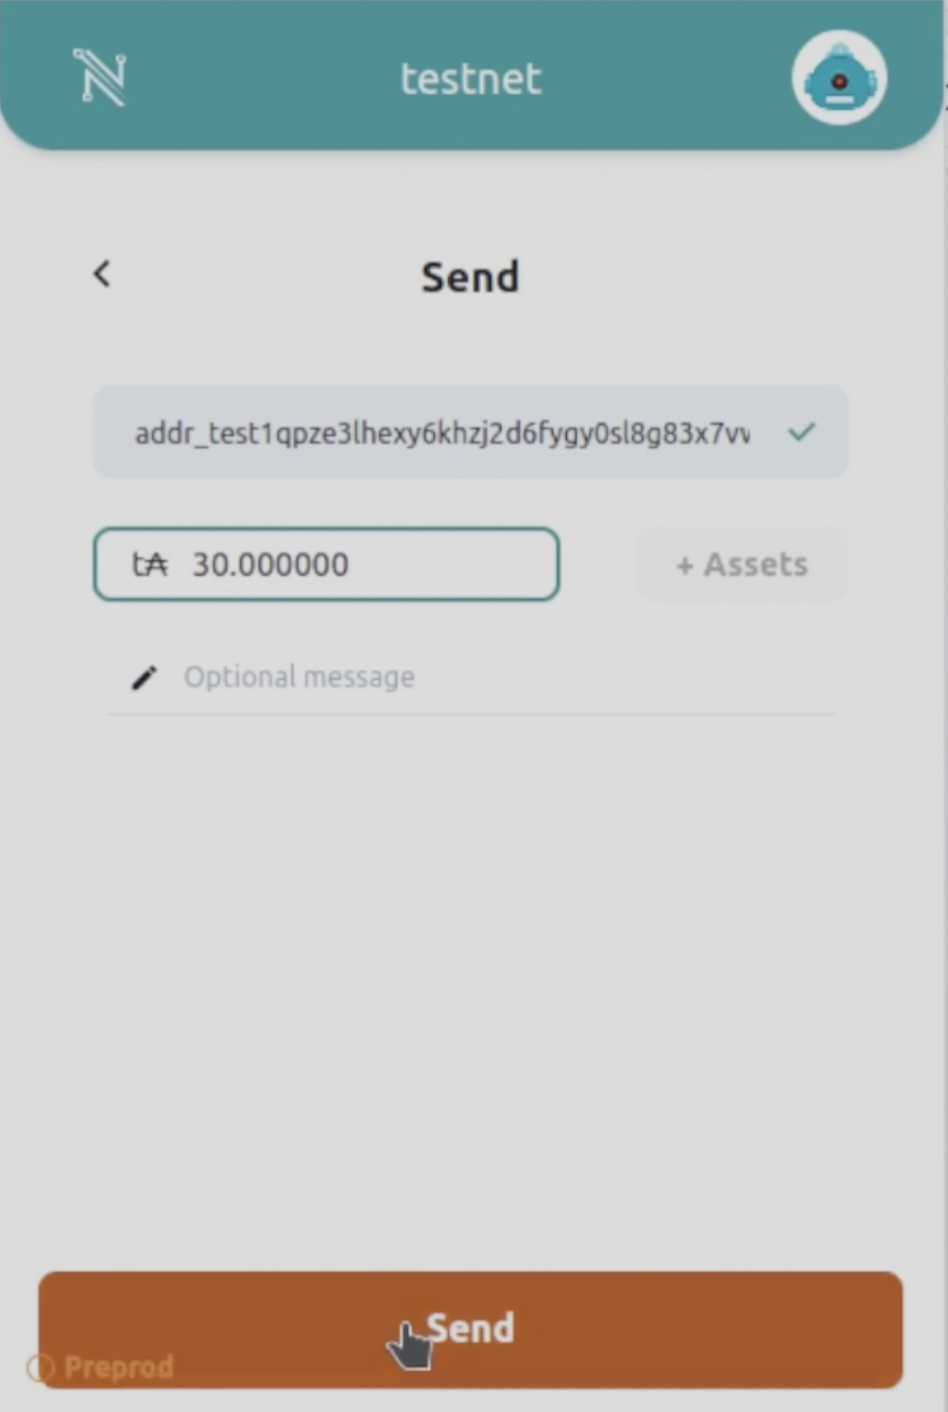
\includegraphics[width=100px]{./imgs/fe2}
        \caption{Nami Wallet with transaction details entered, ready to send}
    \end{figure}
    
    \item \textbf{Viewing the Pending Transaction in History}\\
    Upon receiving the "Transaction submitted" message, we immediately see that the transaction is displayed in the transaction history with a \texttt{Pending} status. At this stage, the transaction has not yet been confirmed on-chain, but it is already recorded in the Nami Wallet’s transaction history as a pending transaction. This early visibility is crucial because it allows us to reference this transaction’s outputs before they are officially confirmed on the blockchain. 
    
    This feature is key to TxChaining: we can now initiate new transactions that use the outputs from this pending transaction as inputs, improving transaction efficiency by removing confirmation wait times between dependent transactions.
    \newline
    \begin{figure}[ht]
        \centering
        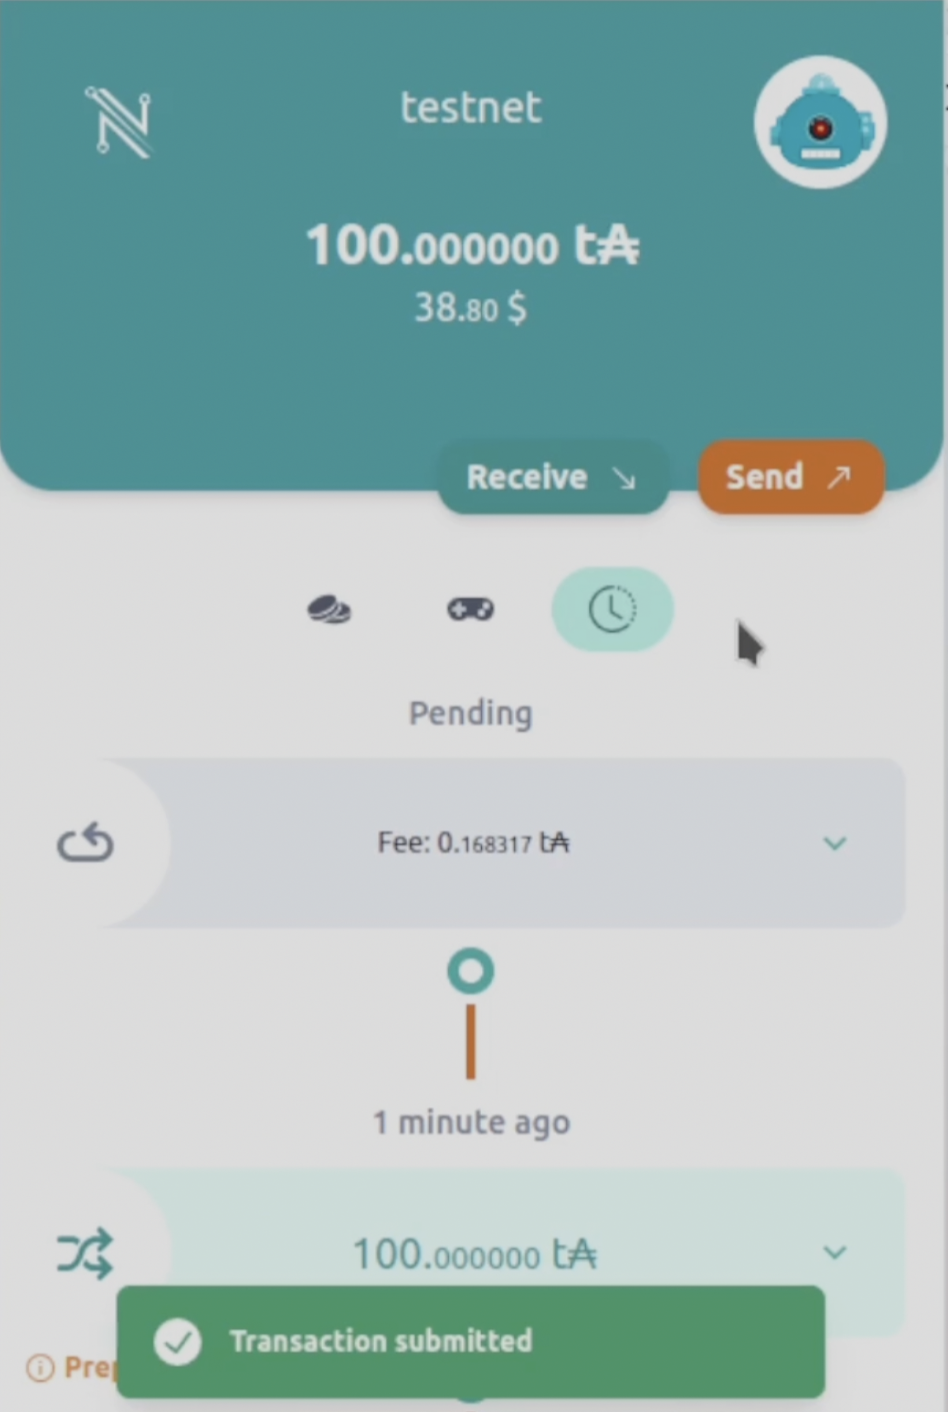
\includegraphics[width=100px]{./imgs/fe3}
        \caption{Nami Wallet transaction history displaying pending transaction}
    \end{figure}
    
    \item \textbf{Accessing Transaction Details and Verifying Outputs}\\
    To further explore this pending transaction, we click on the transaction entry in the history to expand its details. This view provides the transaction hash and relevant output data, which are essential for creating subsequent chained transactions. 

    Additionally, we see a link to CardanoScan, allowing us to track the transaction’s on-chain status once it’s confirmed. Initially, since the transaction is still pending and has not been included in a block, this link will not lead to a transaction page. However, once confirmed, the link becomes active, leading to a full transaction details page on CardanoScan. This approach helps users and developers verify transaction status and outputs seamlessly across the pending and confirmed states.
    \newline
    \begin{figure}[ht]
        \centering
        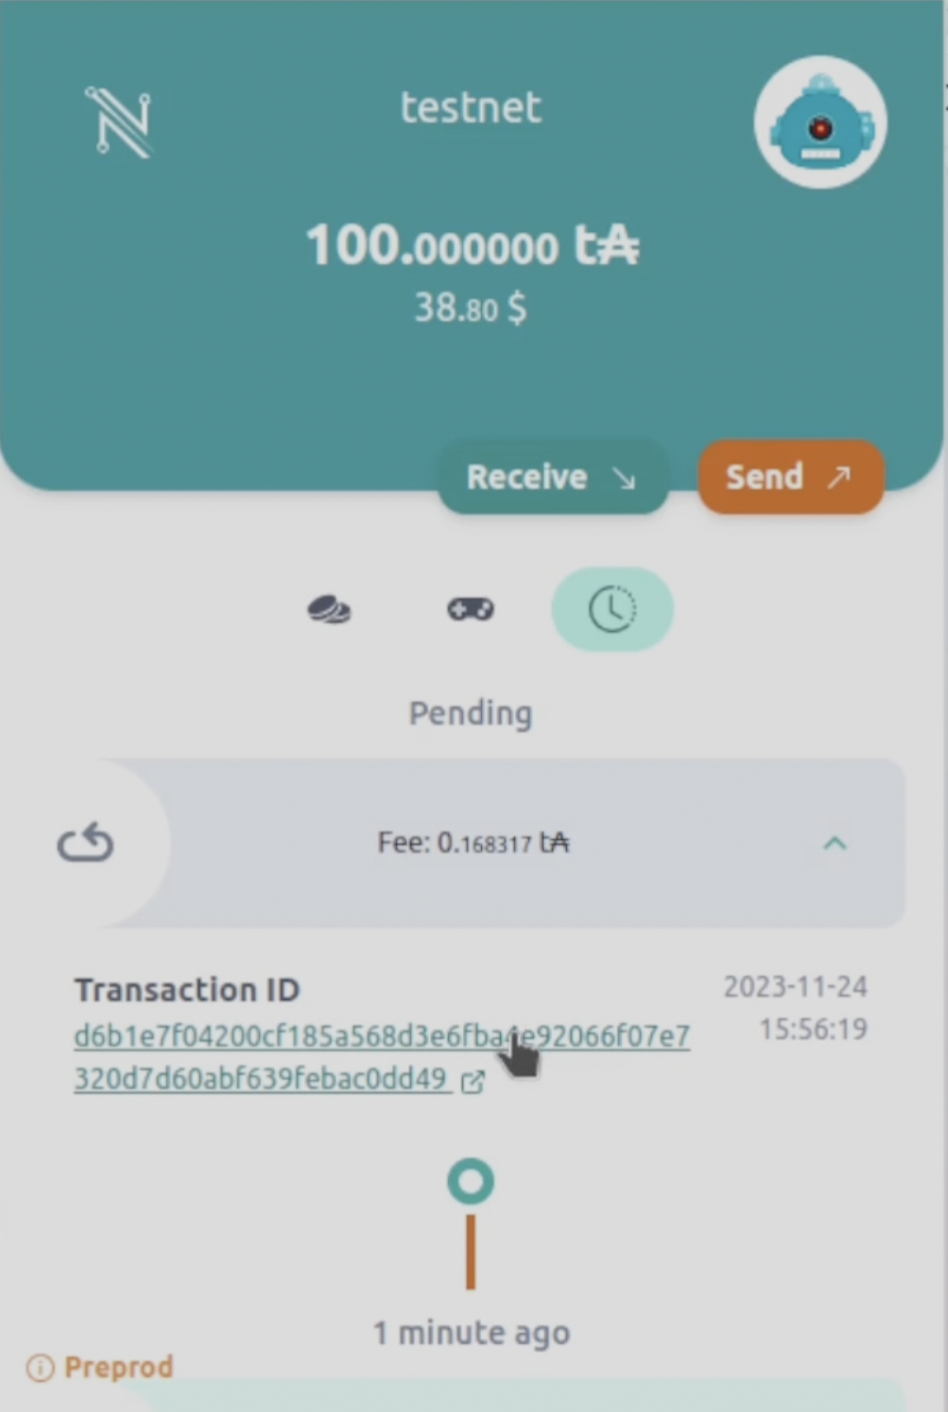
\includegraphics[width=100px]{./imgs/fe4}
        \caption{Expanded transaction details showing transaction hash and CardanoScan link}
    \end{figure}
\end{enumerate}

\subsection{Testing Insights and Results}

Through this testing process, we confirmed that the Nami Wallet’s new TxChaining functionality effectively supports the early use of pending transactions. Specifically:

\begin{itemize}
    \item The modified Nami Wallet can display pending transactions in real-time, showing all relevant details required for subsequent transactions.
    \item Users can leverage transaction outputs from pending transactions, enabling chained transactions without waiting for on-chain confirmation.
\end{itemize}

This testing underscores the functionality and user benefits of TxChaining within the Cardano ecosystem. By enabling rapid, chained transactions, we empower developers and users to interact more fluidly with Cardano-based dApps, ultimately enhancing the blockchain’s efficiency and scalability.

\section{Conclusion}
The implementation of Open Transaction Chaining in the Cardano ecosystem represents a significant leap forward in enhancing transaction efficiency and usability for Cardano dApps. Our work on the Nami Wallet and subsequent documentation provides a foundation for future enhancements and sets a precedent for community-driven innovations in the blockchain space. TxChaining introduces new possibilities for high-frequency and low-latency dApp interactions, and we look forward to continued community support and adoption of these improvements.

\end{document}